%%%%%%%%%%%%%%%%%%%%%%%%%%%%%%%%%%%%%%%%%%%%%%%%%%%%%%%%%%%%%%%%%%%%%%%%%%%%%%%%%%%%%%%%%%%%%%%%
%
% CSCI 1430 Written Questions
%
% This is a LaTeX document. LaTeX is a markup language for producing documents.
% Your task is to answer the questions by filling out this document, then to
% compile this into a PDF document.
% You will then upload this PDF to `Gradescope' - the grading system that we will use.
% Instructions for upload will follow soon.
%
%
% TO COMPILE:
% > pdflatex thisfile.tex
%
% If you do not have LaTeX and need a LaTeX distribution:
% - Departmental machines have one installed.
% - Personal laptops (all common OS): http://www.latex-project.org/get/
%
% If you need help with LaTeX, come to office hours. Or, there is plenty of help online:
% https://en.wikibooks.org/wiki/LaTeX
%
% Good luck!
% James and the 1430 staff
%
%%%%%%%%%%%%%%%%%%%%%%%%%%%%%%%%%%%%%%%%%%%%%%%%%%%%%%%%%%%%%%%%%%%%%%%%%%%%%%%%%%%%%%%%%%%%%%%%
%
% How to include two graphics on the same line:
%
% \includegraphics[width=0.49\linewidth]{yourgraphic1.png}
% \includegraphics[width=0.49\linewidth]{yourgraphic2.png}
%
% How to include equations:
%
% \begin{equation}
% y = mx+c
% \end{equation}
%
%%%%%%%%%%%%%%%%%%%%%%%%%%%%%%%%%%%%%%%%%%%%%%%%%%%%%%%%%%%%%%%%%%%%%%%%%%%%%%%%%%%%%%%%%%%%%%%%

\documentclass[11pt]{article}

\usepackage[english]{babel}
\usepackage[utf8]{inputenc}
\usepackage{amssymb}
\usepackage{xcolor}
\usepackage[colorlinks = true,
            linkcolor = blue,
            urlcolor  = blue]{hyperref}
\usepackage[a4paper,margin=1.5in]{geometry}
\usepackage{stackengine,graphicx}
\usepackage{fancyhdr}
\setlength{\headheight}{15pt}
\usepackage{microtype}
\usepackage{times}
\usepackage[shortlabels]{enumitem}
\setlist[enumerate]{topsep=0pt}
\usepackage{amsmath}

% a great python code format: https://github.com/olivierverdier/python-latex-highlighting
\usepackage{pythonhighlight}

\frenchspacing
\setlength{\parindent}{0cm} % Default is 15pt.
\setlength{\parskip}{0.3cm plus1mm minus1mm}

\pagestyle{fancy}
\fancyhf{}
\lhead{Project 1 Questions}
\rhead{CSCI 1430}
\rfoot{\thepage}

\date{}

\title{\vspace{-1cm}Project 1 Written Questions Solutions}


\begin{document}
\maketitle
\vspace{-3cm}
\thispagestyle{fancy}

\section*{Instructions}
\begin{itemize}
  \item 6 questions.
  \item Include code, images, and equations where appropriate.
  \item Please make this document anonymous.
  \item When you are finished, compile this document to a PDF and submit it directly to Gradescope. On upload, \textbf{Gradescope will ask you to assign question numbers to your pages}. Making each question end with a page break after your answer is a good way to ease this process.
  \item This assignment is \textbf{fixed length}, and the pages have been assigned for you in Gradescope. As a result, \textbf{please do NOT add any new pages}. We will provide ample room for you to answer the questions. If you \emph{really} wish for more space, please add a page \emph{at the end of the document}.
  \item \textbf{We do NOT expect you to fill up each page with your answer.} Some answers will only be a few sentences long, and that is okay.
\end{itemize}

\section*{Questions}

\paragraph{Q1:} Image convolution, a type of image filtering, is a fundamental image processing tool that you will use repeatedly throughout the course.

\begin{enumerate}[(a)]
\item \emph{Explicitly describe} the 3 main components of image convolution:
\begin{enumerate}[(i)]
    \item input
    \item transformation (how it happens)
    \item output
\end{enumerate}
\item Why is image convolution important in Computer Vision? Which applications does it allow?
\end{enumerate}


%%%%%%%%%%%%%%%%%%%%%%%%%%%%%%%%%%%
\paragraph{A1:} Your answer here.
% Uncomment the stencil below and fill in your solution.

% \begin{enumerate}[(a)]
% \item 
% \begin{enumerate}[(i)]
%     \item 
%     \item 
%     \item 
% \end{enumerate}
% \item 
% \end{enumerate}

%%%%%%%%%%%%%%%%%%%%%%%%%%%%%%%%%%%

% Please leave the pagebreak
\pagebreak
\paragraph{Q2:} Correlation is another basic image operation. Correlation and convolution are, in some sense, the simplest operations we can perform to extract information from images.
\begin{enumerate}[(a)]
    \item 
    What is the difference between convolution and correlation?

    \item
    Construct a scenario which produces a different output between both operations. Include the kernel you used and your image results.
    
    \emph{Please use \href{https://docs.scipy.org/doc/scipy/reference/generated/scipy.ndimage.convolve.html}{$scipy.ndimage.convolve$} and \href{https://docs.scipy.org/doc/scipy/reference/generated/scipy.ndimage.correlate.html}{$scipy.ndimage.correlate$} to experiment!}
    
\end{enumerate}


%%%%%%%%%%%%%%%%%%%%%%%%%%%%%%%%%%%
\paragraph{A2:} Your answer here.
% Uncomment the stencil below and fill in your solution.

% \begin{enumerate}[(a)]

% \item 

% \item 

% \end{enumerate}

%%%%%%%%%%%%%%%%%%%%%%%%%%%%%%%%%%%

% Please leave the page break
\pagebreak
\paragraph{Q3:} We create hybrid images by high pass filtering one image, low pass filtering another image, and summing the two images. For (a--c), which filter does the kernel represent? For (d--e), which filter produced the output images?

%%%%%%%%%%%%%%%%%%%%%%%%%%%%%%%%%%%
\emph{LaTeX:} To fill in boxes, replace `\textbackslash square' with `\textbackslash blacksquare' for your answer.

\begin{enumerate}[(a)]
\item
 $\begin{bmatrix}
    1 & 0 & -1 \\
    1 & 0 & -1 \\
    1 & 0 & -1 \\
 \end{bmatrix}$
\begin{tabular}[h]{ll}
$\square$ & High pass \\
$\square$ & Low pass \\
$\square$ & Neither \\
\end{tabular}

\item
 $\begin{bmatrix}
    \frac{1}{9} & \frac{1}{9} & \frac{1}{9} \\
    \frac{1}{9} & \frac{1}{9} & \frac{1}{9} \\
    \frac{1}{9} & \frac{1}{9} & \frac{1}{9}
 \end{bmatrix}$
\begin{tabular}[h]{ll}
$\square$ & High pass \\
$\square$ & Low pass \\
$\square$ & Neither \\
\end{tabular}

\item
$\begin{bmatrix}
    -\frac{1}{9} & -\frac{1}{9} & -\frac{1}{9} \\
    -\frac{1}{9} & \frac{8}{9} & -\frac{1}{9} \\
    -\frac{1}{9} & -\frac{1}{9} & -\frac{1}{9}
  \end{bmatrix}$
\begin{tabular}[h]{ll}
$\square$ & High pass \\
$\square$ & Low pass \\
$\square$ & Neither \\
\end{tabular}

\item
Input image:\\
\raisebox{\baselineskip-\height}{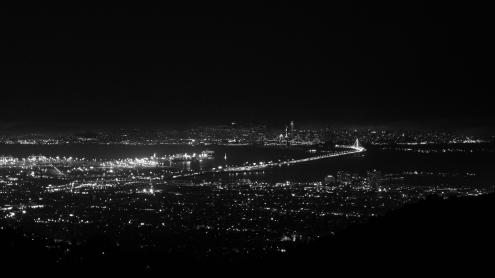
\includegraphics[width = 6cm]{q3img0.png}} \\
Output image 1:\\
\raisebox{\baselineskip-\height}{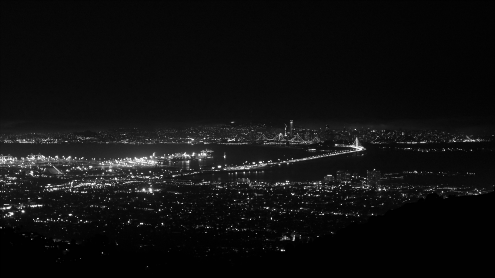
\includegraphics[width = 6cm]{q3img1.png}}
\begin{tabular}[h]{lc}
$\square$ & High pass \\
$\square$ & Low pass \\
\end{tabular}

\item
Output image 2:\\
\raisebox{\baselineskip-\height}{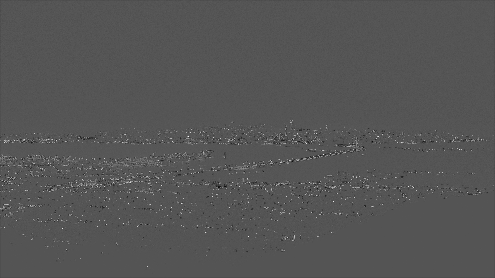
\includegraphics[width = 6cm]{q3img2.png}}
\begin{tabular}[h]{lc}
$\square$ & High pass \\
$\square$ & Low pass \\
\end{tabular}

\item
Which of the following statements are true? (Check all that apply).

\begin{tabular}[h]{ll}
$\square$ & High pass filter kernels will always contain at least one negative number \\
$\square$ & A Gaussian filter is an example of a low pass filter \\
$\square$ & A high pass filter is the basis for most smoothing methods \\
$\square$ & In a high pass filter, the center of the kernel must have the highest value \\
\end{tabular}

\end{enumerate}



%%%%%%%%%%%%%%%%%%%%%%%%%%%%%%%%%%%

% Please leave the pagebreak
\pagebreak
\paragraph{Q4:} 
\begin{enumerate}[(a)]
    \item 
    How does computation time vary with filter sizes from $3\times3$ to $15\times15$ (test odd and square sizes, i.e. $3\times3$, $5\times5$, $7\times7$, etc.), and with image sizes from approximately 0.25 to 8 megapixels? To find out fill out the below stencil to graph, for each of the above filter sizes, the correlation between an image size (x-axis) and time to convolve/correlate (y-axis) that image– each filter size should be its own line in the multi-line plot. 
    
    The stencil code imports the libraries you will need, but to understand how to use them you must look at the documentation.
    \begin{itemize}
    \item convolve/correlate - \href{https://docs.scipy.org/doc/scipy/reference/generated/scipy.ndimage.convolve.html}{$scipy.ndimage.convolve$} or \href{https://docs.scipy.org/doc/scipy/reference/generated/scipy.ndimage.correlate.html}{$scipy.ndimage.correlate$}
    \item rescale - \href{https://scikit-image.org/docs/dev/api/skimage.transform.html#skimage.transform.rescale}{$skimage.transform.rescale$}
    \item resize - \href{https://scikit-image.org/docs/dev/api/skimage.transform.html#skimage.transform.resize}{$skimage.transform.resize$}
    \item rescale vs resize (and an example) \href{http://scikit-image.org/docs/dev/auto_examples/transform/plot_rescale.html}{here}
    \end{itemize} 

    
    Add your graph as well as a brief description of what your graph demonstrates, below.

\emph{Note A megapixel is 1,048,576 ($2^20$) pixels (1024$\times$1024), or sometimes also 1,000,000 pixels (especially if you manufacture cameras). Megapixels is often shortened to MP or MPix.}

\emph{Image:} \href{RISDance.jpg}{RISDance.jpg} (in the .tex directory).

\begin{python}
import time 
import matplotlib.pyplot as plt
from skimage import io, img_as_float32
#use to rescale+resize image
from skimage.transform import rescale, resize
#use to convolve/correlate image
from scipy.ndimage import correlate

#This reads in image and converts to a floating point format
# 1) TODO - replace PATH with the actual path to the 
#    downloaded RISDance.jpg image linked above
image = img_as_float32(io.imread('PATH'))

# 2) TODO - change the image size so it starts at 8MPix 
#    use one of the imported libraries
original_image = 

# 3) TODO - iterate through odd numbers from 3 to 15
#   (inclusive!!) these will represent your filter sizes
#   (3x3,5x5,7x7, etc.), for each filter size you will...
for kernel_size in range():

    #because for each loop you are resizing your image, you 
    #want to start each loop w/the original image size
    shrinking_image = original_image 
    
    #these lists will hold the values you plot
    image_sizes = [] #x axis
    times = [] #y axis

    #while image size is bigger than .25MPx
    while(shrinking_image.size > 250000):
    
    	# 4) TODO - create your kernel. Your kernel can hold
    	#    any values, as the kernel values shouldn't 
    	#    affect computation time. The size of the kernel
    	#    must be kernel_size x kernel_size
        kernel = 
        
        #5) TODO - reduce your image size. You can choose by 
        # what increments to reduce your image.
        shrinking_image = 
        
        #gets the current time (in seconds)
        start = time.time() 
        
        # 6) TODO - use one of the imported libraries to do 
        # your correlation/convolution on the image. You can 
        # choose which operation to perform.
        
        
        #gets the current time (in seconds)
        end = time.time() 
        
        #7) TODO - figure out what values to append, and 
        #   append them here
        image_sizes.append()
        times.append()
    
    #each filter size will be plotted as a separate line, in 
    #a multi-line 2-dimensional graph
    plt.plot(times, image_sizes, label=str(kernel.size))

#plot
plt.axes().set_xlabel('image size (pixels)')
plt.axes().set_ylabel('operation time (seconds)')
plt.legend(title="filter sizes (pixels)")
plt.show()

\end{python}


\item
    Do the results match your expectation given the number of multiply and add operations in convolution?
\end{enumerate}

%%%%%%%%%%%%%%%%%%%%%%%%%%%%%%%%%%%
\paragraph{A4:} Your answer here.
% Uncomment the stencil below and fill in your solution.

% \begin{enumerate}[(a)]

% \item 

% \item 

% \end{enumerate}

%%%%%%%%%%%%%%%%%%%%%%%%%%%%%%%%%%%
\pagebreak 
\paragraph{Q5:} The upcoming coding assignment requires the extensive use of the library numpy, which handles computation with large, multi-dimensional arrays and matrices. Here are some small exercises on basic numpy operations to get you started! Write \emph{one} numpy function to complete each of the following tasks.

Note that numpy is usually imported as
\begin{verbatim}
    import numpy as np
\end{verbatim}
at the top of the code file. You can then call numpy functions with \begin{verbatim}
    np.function_name()
\end{verbatim}
You are encouraged to test out your answers by creating your own python program, importing numpy and calling and printing the results of your solutions!

\begin{enumerate}[a.]
    \item Create an array of shape (320,640) filled with zeros.
    \item Given a variable called \emph{img} of shape (1, 1, 320, 640), create a new 2D array variable of shape (320, 640) from \emph{img}, i.e. remove all the 1-sized dimensions. 
    \item Conversely, say you have an array variable \emph{img} of shape (320, 640), create a new 2D array variable of shape (1, 320, 640) from \emph{img}, i.e. add a dimension. 
    \item Pad an \textbf{RGB} (remember, this means the image has 3 channels) image array, \emph{img}, with two zeros on either side of each row and 3 zeros values on either side of each column. Don't add zeros to the front or back (the color channel dimension).
    \item Clip the image array, \emph{img}, so all its values lie within the range [-0.5, 0.5].
    \item With an RGB-image array, \emph{img}, of shape (320, 640, 3), retrieve the blue channel of the image while preserving all of \emph{img}'s dimensions and values. 
    \item With an RGB-image array, \emph{img}, of shape (320, 640, 3), retrieve the red and blue channels of the image. 
\end{enumerate}


%%%%%%%%%%%%%%%%%%%%%%%%%%%%%%%%%%%
\paragraph{A5:} Your answer here
%  Uncomment the stencil below and fill in your solution.

% \begin{enumerate}[(a)]
% \item 
% \item 
% \item 
% \item 
% \item 
% \item 
% \item 
% \end{enumerate}


%%%%%%%%%%%%%%%%%%%%%%%%%%%%%%%%%%%
% Please leave the pagebreak
\pagebreak
\paragraph{Q5:} 
In 1990, \emph{New York Times} photography critic Andy Grundberg \href{https://www.nytimes.com/1990/08/12/arts/photography-view-ask-it-no-questions-the-camera-can-lie.html}{stated that:}\\``In the future, readers of newspapers and
magazines will probably view news pictures more as
illustrations than as reportage, since they can no longer distinguish between a genuine image and one that has been manipulated.''

\begin{enumerate}[(a)]
    \item When is Grundberg's `future' ? Why? (2--4 sentences)
    
    \item When is a news picture no longer genuine? Are any manipulations permissible, and if so, which ones? (2--4 sentences)
    
    \item If you worked for the \emph{New York Times} and were tasked with maintaining readers' trust in news pictures in Grundberg's future, what would you do? Consider everything that happens in the publication of a news picture. Describe your approach, and why it would work. (3--5 sentences)
    
    \begin{enumerate}[(i)]
    \item As per c), but instead you worked for the \emph{College Hill Independent}? \\(2--4 sentences)
    \end{enumerate}
    
    \item Include an cited example of a manipulated news picture, and identify the manipulation. What was the intent and impact of the manipulation? (2--4 sentences)
\end{enumerate}

\emph{Note:} These are open questions. We will grade for thought and justification. 

%%%%%%%%%%%%%%%%%%%%%%%%%%%%%%%%%%%

 \paragraph{A6:} Your answer here
%  Uncomment the stencil below and fill in your solution.
% \begin{enumerate}[(a)]
% \item
% \item 
% \item 
% \begin{enumerate}[(i)]
%     \item
% \end{enumerate}
% \item
% \end{enumerate}


%%%%%%%%%%%%%%%%%%%%%%%%%%%%%%%%%%%

%% any suggestions for more? 
\pagebreak
\section*{Feedback? (Optional)}
Please help us make the course better. If you have any feedback for this assignment, we'd love to hear it!

\end{document}